% belief_control_integration.tex
% Supplementary material addressing Major Weakness #2 from THRI-2025-0214 reviews.
%
% Provides a precise, code-grounded description of:
%   (i)   How belief representations are incorporated into action selection
%   (ii)  How training data is collected in both stages
%   (iii) How the framework components are integrated
%   (iv)  Variable-level data flow at each timestep
%
% Intended to be incorporated into the revised manuscript (Sections 3.x or new Appendix).

\documentclass[11pt]{article}
\usepackage[margin=1in]{geometry}
\usepackage{amsmath,amssymb,amsfonts}
\usepackage{algorithm}
\usepackage{algpseudocode}
\usepackage{booktabs}
\usepackage{tikz}
\usetikzlibrary{arrows.meta,positioning,calc,fit,backgrounds}
\usepackage{hyperref}
\usepackage{xcolor}

\newcommand{\bvec}{\mathbf{b}_t}
\newcommand{\svec}{\mathbf{s}_t}
\newcommand{\cvec}{\mathbf{c}_t}
\newcommand{\hvec}{\mathbf{h}_t}
\newcommand{\wvec}{\mathbf{w}_t}
\newcommand{\avec}{\mathbf{a}_t}
\newcommand{\goalset}{\mathcal{G}}
\newcommand{\real}{\mathbb{R}}

\title{BRACE: Detailed Integration of Belief Inference and \\Assistance Arbitration\\[0.5em]
\large Supplementary Clarification for Major Weakness~2}
\author{Response to THRI-2025-0214 Reviews}
\date{}

\begin{document}
\maketitle
\thispagestyle{empty}

%% =================================================================
\section{Overview}
%% =================================================================

This document provides a precise, implementation-grounded specification of how the BRACE framework integrates its Bayesian belief inference module with the reinforcement-learning-based arbitration policy.
It is organized around the four specific ambiguities identified by the reviewers:
\begin{enumerate}
    \item How belief representations are incorporated into action selection (\S\ref{sec:belief-to-action}).
    \item How training data is collected and used across the two training stages (\S\ref{sec:training-data}).
    \item How the framework components (Bayesian inference, expert policy, arbitration policy, simulated human) are integrated into a single pipeline (\S\ref{sec:integration}).
    \item A step-by-step, variable-level data-flow specification for a single timestep (\S\ref{sec:dataflow}).
\end{enumerate}

\noindent Throughout, we use the following notation consistently:
\begin{center}
\begin{tabular}{@{}cl@{}}
\toprule
Symbol & Definition \\
\midrule
$\goalset = \{g_1, \ldots, g_N\}$ & Set of $N$ candidate goal positions \\
$g^*$ & True (hidden) goal, unknown to the system \\
$\svec \in \real^d$ & Environment state (EE position, velocity, relative object/obstacle positions) \\
$\bvec \in \Delta^{N-1}$ & Belief: probability simplex over $\goalset$ at time $t$ \\
$\cvec(\svec)$ & Context features extracted from $\svec$ (minimum obstacle distance) \\
$\hvec \in \real^2$ & Raw human velocity command at time $t$ \\
$\wvec \in \real^3$ & Expert policy action $[v_x, v_y, \text{gripper}]$ \\
$\gamma_t \in [0,1]$ & Assistance blending parameter (output of the arbitration policy) \\
$\avec$ & Executed action: $\avec = (1 - \gamma_t)\,\hvec + \gamma_t\,\wvec$ \\
$\phi$ & Learnable parameters of the Bayesian inference module \\
$\theta$ & Learnable parameters of the PPO arbitration policy \\
\bottomrule
\end{tabular}
\end{center}


%% =================================================================
\section{How Belief Is Incorporated into Action Selection}
\label{sec:belief-to-action}
%% =================================================================

The belief vector $\bvec$ influences the executed action through two distinct pathways.

\subsection{Pathway 1: Arbitration Policy Input}

The arbitration policy $\pi_\theta$ receives a \emph{fused observation} formed by concatenating the environment state $\svec$ with the full belief vector $\bvec$:
\begin{equation}
    \mathbf{o}_t = [\,\svec \;\|\; \bvec\,] \;\in\; \real^{d + N}
    \label{eq:fused-obs}
\end{equation}
This fused vector is the sole input to the PPO actor-critic network.  The actor head outputs a scalar $\tilde{\gamma}_t \in [-1,1]$ (via $\tanh$ activation), which is mapped to the blending parameter:
\begin{equation}
    \gamma_t = \tfrac{1}{2}(\tilde{\gamma}_t + 1) \;\in\; [0,1]
    \label{eq:gamma-map}
\end{equation}
Crucially, the policy sees the \emph{entire} probability distribution $\bvec$, not just the MAP estimate $\hat{g} = \arg\max_i b_t(g_i)$.
This enables the policy to distinguish, for example, a state where one goal has $p = 0.95$ (high confidence $\Rightarrow$ strong assistance is safe) from a state where three goals each have $p \approx 0.33$ (high ambiguity $\Rightarrow$ assistance risks guiding toward the wrong goal).

The state vector $\svec$ includes context features $\cvec(\svec)$---specifically, the minimum distance from the end-effector to the nearest obstacle and the normalized progress toward each candidate goal.
These context features, together with $\bvec$, allow the policy to jointly condition assistance on both \emph{intent uncertainty} and \emph{environmental constraint severity}, as required by Theorem~1.

\subsection{Pathway 2: Expert Goal Selection at Deployment}

The expert policy $\pi_{\text{expert}}$ provides optimal actions toward a \emph{single} goal.
During training and deployment, the expert's target is determined differently:

\begin{itemize}
    \item \textbf{Training:} The expert always receives the true goal $g^*$ (via a one-hot encoding appended to its observation).
    This is possible because the training environment has oracle access to the hidden goal.
    The expert acts as an ideal oracle: it provides the best possible action \emph{if} the true goal were known with certainty.

    \item \textbf{Deployment:} The true goal is unknown.  The expert targets the MAP goal derived from the belief:
    \begin{equation}
        \hat{g}_t = g_{\arg\max_i \, b_t(g_i)}
    \end{equation}
    The expert then computes $\wvec = \pi_{\text{expert}}(\svec, \hat{g}_t)$.
\end{itemize}

\noindent\textbf{Important clarification:} We do \emph{not} compute a belief-weighted mixture of per-goal expert actions.
Instead, the belief influences action selection in two complementary ways:
(i)~$\gamma_t$ is conditioned on the full belief to modulate \emph{how much} of the expert's action to use, and
(ii)~the expert's target goal is the MAP estimate from the belief.
When belief entropy is high (ambiguous intent), the policy learns to reduce $\gamma_t$, which attenuates the expert's potentially incorrect guidance.
When the belief concentrates on the true goal, $\gamma_t$ increases, amplifying correct expert assistance.


\subsection{Final Blended Action}

Given $\hvec$ (human input), $\wvec$ (expert action), and $\gamma_t$ (assistance level), the executed action is:
\begin{equation}
    \avec = (1 - \gamma_t)\,\hvec + \gamma_t\,\wvec
    \label{eq:blend}
\end{equation}
This linear blending ensures smooth interpolation between full human control ($\gamma_t = 0$) and full expert control ($\gamma_t = 1$).
The action $\avec$ is applied to the environment, producing the next state $\mathbf{s}_{t+1}$.


%% =================================================================
\section{Training Data Collection and Distribution}
\label{sec:training-data}
%% =================================================================

Training occurs in two sequential stages, each with a distinct data-collection process.
Below we describe each stage, the behavior distribution the belief module observes, and how the transition between stages is handled.

\subsection{Stage 1: Belief Module Pretraining (Supervised)}

\textbf{Data generation.}
We generate $M = 5{,}000$ synthetic trajectories of length $T = 100$ timesteps.
Each trajectory is produced by the simulated human model operating \emph{without any assistance} ($\gamma = 0$):
\begin{enumerate}
    \item Sample $N$ goal positions uniformly within the workspace bounds.
    \item Randomly select one goal as $g^*$.
    \item Initialize the end-effector at a random starting position.
    \item For $t = 1, \ldots, T$:
    \begin{itemize}
        \item The simulated human computes a deterministic minimum-jerk direction toward $g^*$.
        \item Potential-field obstacle avoidance adjusts the direction near obstacles.
        \item AR(1) pink noise (amplitude 3.2\%, AR coefficient 0.5) is added to simulate motor variability.
        \item The noisy action $\hvec$ is applied directly to the environment (no blending).
    \end{itemize}
\end{enumerate}

\textbf{Optimization objective.}
The belief module parameters $\phi = \{\beta, w_\theta, w_d\}$ (constrained positive via softplus) are optimized to minimize the negative log-likelihood of the true goal:
\begin{equation}
    \mathcal{L}_{\text{supervised}}(\phi) = -\frac{1}{M}\sum_{m=1}^{M}\frac{1}{T}\sum_{t=1}^{T} \log P_\phi(g^* \mid \mathbf{x}_{1:t}, \mathbf{h}_{1:t})
    \label{eq:sup-loss}
\end{equation}
where the posterior $P_\phi(g^* \mid \cdot)$ is obtained by recursive Bayesian filtering starting from a uniform prior.

\textbf{Behavior distribution.}
During pretraining, the belief module observes trajectories generated under \emph{unassisted} human control.
The positional trajectory $\mathbf{x}_{1:T}$ reflects the simulated human's noisy goal-directed behavior without expert intervention.

\subsection{Stage 2: Joint Arbitration Training (RL + Belief Fine-tuning)}

\textbf{On-policy data collection.}
The arbitration policy is trained using PPO.
At each timestep of each rollout episode, the environment executes the following procedure (Algorithm~\ref{alg:brace-step}):
\begin{enumerate}
    \item The simulated human produces $\hvec$ given the \emph{current} EE position and the true goal.
    \item The Bayesian module updates $\bvec$ given $\hvec$, the current EE position, and goal positions.
    \item The fused observation $\mathbf{o}_t = [\svec \| \bvec]$ is returned to the PPO policy.
    \item The PPO policy outputs $\gamma_t$.
    \item The expert produces $\wvec$ (toward the true goal during training).
    \item The blended action $\avec = (1 - \gamma_t)\hvec + \gamma_t \wvec$ is executed.
    \item The environment transitions to $\mathbf{s}_{t+1}$.
    \item The arbitration reward is computed (Eq.~\ref{eq:reward}).
\end{enumerate}

\textbf{Key distributional considerations.}

\begin{itemize}
    \item \textbf{Human model does not adapt to assistance:}
    The simulated human is a \emph{fixed} model that always computes its action based on the current EE position and the true goal.
    It does not observe or react to the assistance level $\gamma_t$ or the expert action $\wvec$.
    This means the human behavior distribution $P(\hvec \mid \mathbf{x}_t, g^*)$ is identical in both training stages.
    The belief module's likelihood model $P_\phi(\hvec \mid \mathbf{x}_t, g_i)$ therefore remains well-specified: the same noisy-rational model applies regardless of the assistance context.

    \item \textbf{Positional distribution shifts between stages:}
    Although the human action distribution is invariant, the \emph{positional} distribution of the EE trajectory $\mathbf{x}_{1:T}$ changes between stages.
    During pretraining, positions follow unassisted human trajectories.
    During joint training, the blended action $\avec$ produces different positional dynamics---typically smoother, more direct paths.
    The belief module conditions its likelihood on both $\hvec$ and $\mathbf{x}_t$, so it encounters positions it did not see during pretraining.
    This is precisely why joint fine-tuning (Stage~2) is necessary: it adapts the belief module's parameters to the positional distribution induced by the assistance policy.

    \item \textbf{Belief updates condition on raw human input, not blended action:}
    The Bayesian module receives the \emph{raw} human velocity command $\hvec$, not the executed blended action $\avec$.
    This design choice ensures that the likelihood computation $P(\hvec \mid \mathbf{x}_t, g_i)$ directly models human intent, uncontaminated by the expert's contribution.
    The blended action only affects the next state $\mathbf{s}_{t+1}$ (and thus the next EE position for the subsequent belief update).
\end{itemize}


\subsection{End-to-End Gradient Flow for Belief Fine-tuning}

During Stage~2, the belief module parameters $\phi$ are jointly optimized alongside the policy parameters $\theta$ using a mixed objective that gradually shifts from supervised to reinforcement-driven:
\begin{equation}
    \mathcal{L}_{\text{total}}(\theta, \phi) = \alpha\, \mathcal{L}_{\text{RL}}(\theta, \phi) + (1 - \alpha)\, \mathcal{L}_{\text{supervised}}(\phi)
    \label{eq:mixed-obj}
\end{equation}
where $\alpha$ is annealed from 0.3 to 0.9 over 500{,}000 timesteps.

The RL gradient with respect to $\phi$ is estimated via REINFORCE:
\begin{equation}
    \nabla_\phi \mathcal{L}_{\text{RL}} \approx \mathbb{E}_\tau \left[ \sum_{t=0}^{T} A_t \, \nabla_\phi \log P_\phi(\bvec \mid \mathbf{x}_{1:t}, \mathbf{h}_{1:t}) \right]
    \label{eq:reinforce}
\end{equation}
where $A_t = R_t - V_\theta(\svec)$ is the advantage estimate (using the PPO critic as baseline).

This gradient flow means that if a particular belief allocation causes the arbitration policy to intervene at the wrong time (increasing task regret), the resulting negative advantage signal pushes the belief parameters to reshape their probability assignments.
For example, if the belief module assigns high confidence prematurely in an ambiguous scenario, causing the policy to assist too aggressively toward the wrong goal, the negative reward signal propagates back to adjust $\beta$, $w_\theta$, and $w_d$ to produce more cautious (higher-entropy) beliefs in similar states.

Stabilization techniques for this gradient include:
\begin{itemize}
    \item \textbf{Advantage baseline:} The critic $V_\theta(\svec)$ serves as a state-dependent baseline, centering the REINFORCE gradient to reduce variance.
    \item \textbf{Gradient clipping:} The L2 norm of $\nabla_\phi \mathcal{L}_{\text{RL}}$ is clipped to $C_{\text{clip}} = 1.0$, preserving gradient direction while bounding magnitude.
    \item \textbf{Confidence-scaled updates:} When the maximum belief probability $p_{\max} < c = 0.8$, the update step is damped by a factor $\alpha_{\text{damp}} = p_{\max} / c$, preventing policy oscillation under high belief uncertainty.
    \item \textbf{Temperature annealing:} The softmax temperature $\tau$ in the belief update is exponentially decayed from 1.0 to 0.1, gradually sharpening beliefs to provide stronger training signal.
\end{itemize}


%% =================================================================
\section{Component Integration}
\label{sec:integration}
%% =================================================================

BRACE consists of four independently defined components that are integrated through the arbitration training environment.  Table~\ref{tab:components} summarizes each component's role, inputs, outputs, and trainability.

\begin{table}[h]
\centering
\caption{BRACE component specification}
\label{tab:components}
\small
\begin{tabular}{@{}p{3.2cm}p{3.0cm}p{3.5cm}p{3.2cm}@{}}
\toprule
\textbf{Component} & \textbf{Input} & \textbf{Output} & \textbf{Training} \\
\midrule
Bayesian Inference Module ($\phi$)
& $\hvec$, $\mathbf{x}_t$, $\{g_i\}$, $\mathbf{b}_{t-1}$
& $\bvec \in \Delta^{N-1}$, loss term
& Stage~1: supervised NLL; Stage~2: mixed NLL + REINFORCE \\
\addlinespace
Arbitration Policy ($\theta$)
& $\mathbf{o}_t = [\svec \| \bvec]$
& $\gamma_t \in [0,1]$, $V(\svec)$
& Stage~2: PPO (actor-critic) \\
\addlinespace
Expert Policy (frozen)
& $\svec$, true goal (train) or MAP goal (deploy)
& $\wvec \in [-1,1]^3$
& Pre-trained SAC; frozen during Stages~1--2 \\
\addlinespace
Simulated Human (fixed)
& $\mathbf{x}_t$, $g^*$, obstacles
& $\hvec \in [-1,1]^2$
& Not learned; calibrated from human data \\
\bottomrule
\end{tabular}
\end{table}


\subsection{Observation Space Construction}

The arbitration policy's observation $\mathbf{o}_t$ is a $(d + N)$-dimensional vector constructed as follows.
For the default configuration ($N = 3$ goals, $K$ obstacles):

\begin{equation}
    \mathbf{o}_t = \bigl[\;
    \underbrace{\mathbf{x}_t}_{\text{EE pos (2)}} \;\big\|\;
    \underbrace{\dot{\mathbf{x}}_t}_{\text{EE vel (2)}} \;\big\|\;
    \underbrace{g_{\text{grip}}}_{\text{gripper (1)}} \;\big\|\;
    \underbrace{\Delta g_1, \ldots, \Delta g_N}_{\text{rel. goals (2N)}} \;\big\|\;
    \underbrace{\Delta o_1, \ldots, \Delta o_K}_{\text{rel. obstacles (2K)}} \;\big\|\;
    \underbrace{d_{\min}^{\text{obs}}}_{\text{nearest obs. (1)}} \;\big\|\;
    \underbrace{p_1, \ldots, p_N}_{\text{goal progress (N)}} \;\big\|\;
    \underbrace{b_t(g_1), \ldots, b_t(g_N)}_{\text{belief (N)}}
    \;\bigr]
    \label{eq:obs-full}
\end{equation}
where $\Delta g_i = g_i - \mathbf{x}_t$ are relative goal positions, $\Delta o_j = o_j - \mathbf{x}_t$ are relative obstacle positions, and $p_i = 1 - \|g_i - \mathbf{x}_t\| / d_{\text{diag}}$ is normalized progress.

\subsection{Arbitration Reward Function}

The PPO policy is trained to maximize the following reward, which couples belief quality with task performance:
\begin{equation}
    R_t = \underbrace{-w_{\text{coll}} \cdot \mathbf{1}_{\text{collision}}}_{\text{safety}}
    + \underbrace{w_{\text{prox}} \cdot \gamma_t \cdot p_{\max} \cdot \mathbf{1}_{\text{near}}}_{\text{assist near target}}
    - \underbrace{w_{\text{far}} \cdot \gamma_t \cdot \mathbf{1}_{\text{far}}}_{\text{penalize premature assist}}
    + \underbrace{w_{\text{prog}} \cdot p_{\max} \cdot (d_{t-1} - d_t)}_{\text{goal progress}}
    - \underbrace{w_{\text{auto}} \cdot \gamma_t^2}_{\text{agency preservation}}
    + \underbrace{w_{\text{goal}} \cdot \log p_{\text{true}}}_{\text{belief accuracy}}
    \label{eq:reward}
\end{equation}
where $p_{\max} = \max_i b_t(g_i)$ is the peak belief probability and $p_{\text{true}} = b_t(g^*)$ is the belief assigned to the true goal.

This reward function creates the coupling between belief quality and control:
\begin{itemize}
    \item The $\log p_{\text{true}}$ term directly rewards accurate goal inference, providing a supervised signal to the belief module during joint training.
    \item The $p_{\max}$-weighted progress term means that task progress is only rewarded when the belief is confident, encouraging the policy to wait for clear intent signals before assisting.
    \item The $\gamma_t^2$ penalty ensures minimal intervention by default, protecting user agency.
    \item The proximity and far-distance indicator terms implement context-dependent assistance: help is rewarded near the believed target and penalized far from all targets.
\end{itemize}

\subsection{Curriculum Progression}

Training proceeds through five curriculum stages that progressively introduce complexity:

\begin{center}
\small
\begin{tabular}{@{}clccp{5cm}@{}}
\toprule
Stage & Name & Goals & Obstacles & Advancement Criterion \\
\midrule
1 & Basic reaching & 1 & 0 & $\geq$100 episodes, success $\geq$80\% \\
2 & Collision avoidance & 1 & 3 & $\geq$200 episodes, success $\geq$75\%, collisions $\leq$15\% \\
3 & Challenging obstacles & 1 & 4 & $\geq$300 episodes, success $\geq$70\% \\
4 & Goal ambiguity & 3 & 3 & $\geq$400 episodes, success $\geq$65\% \\
5 & Full complexity & 3 & 4 & Reward plateau (200-episode window) \\
\bottomrule
\end{tabular}
\end{center}

Stages~1--3 introduce environmental constraints without goal ambiguity, allowing the policy to learn context-aware assistance before facing intent uncertainty.
Stage~4 introduces multiple goals, activating the belief module's role in the observation.
Stage~5 combines both challenges.
This progression ensures stable training: the belief-conditioning pathway is already embedded in the observation from Stage~1 (as a trivially certain 1-goal belief), so the policy gradually learns to use increasingly informative belief signals.


%% =================================================================
\section{Per-Timestep Data Flow}
\label{sec:dataflow}
%% =================================================================

Algorithm~\ref{alg:brace-step} specifies the exact sequence of operations at each timestep during arbitration training, making all variable dependencies explicit.

\begin{algorithm}[h]
\caption{BRACE: single-timestep execution during arbitration training}
\label{alg:brace-step}
\begin{algorithmic}[1]
\Require Current state $\svec$, prior belief $\mathbf{b}_{t-1}$, true goal $g^*$, trained expert $\pi_{\text{expert}}$
\Ensure Next state $\mathbf{s}_{t+1}$, reward $R_t$, updated belief $\bvec$, fused obs.\ $\mathbf{o}_{t+1}$

\Statex \textbf{--- Human Action ---}
\State $\hvec \gets \textsc{SimulatedHuman}(\mathbf{x}_t,\; g^*,\; \text{obstacles})$
    \Comment{min-jerk + obstacle avoidance + AR(1) noise}

\Statex \textbf{--- Belief Update ---}
\State $\ell_i \gets \exp\bigl(-\beta\,[w_\theta \cdot \theta_{\text{dev}}(\hvec, \mathbf{x}_t, g_i) + w_d \cdot d_{\text{dev}}(\hvec, \mathbf{x}_t, g_i)]\bigr)$ \quad for each $g_i \in \goalset$
\State $\bvec^{\text{raw}}(g_i) \gets \text{softmax}\Bigl(\frac{\log b_{t-1}(g_i) + \log \ell_i}{\tau}\Bigr)$
    \Comment{Bayes rule with temperature}
\State $\bvec(g_i) \gets \alpha_{\text{ema}} \cdot \bvec^{\text{raw}}(g_i) + (1 - \alpha_{\text{ema}}) \cdot b_{t-1}(g_i)$
    \Comment{EMA smoothing ($\alpha_{\text{ema}} = 0.85$)}

\Statex \textbf{--- Arbitration Policy ---}
\State $\mathbf{o}_t \gets [\svec \;\|\; \bvec]$
    \Comment{fuse state with belief (Eq.~\ref{eq:obs-full})}
\State $\tilde{\gamma}_t, V_t \gets \pi_\theta(\mathbf{o}_t)$
    \Comment{PPO actor: $\tilde{\gamma}_t \in [-1,1]$; critic: $V_t$}
\State $\gamma_t \gets \tfrac{1}{2}(\tilde{\gamma}_t + 1)$
    \Comment{map to $[0,1]$}

\Statex \textbf{--- Expert Action ---}
\State $\mathbf{o}_t^{\text{expert}} \gets [\svec \;\|\; \text{onehot}(g^*)]$
    \Comment{expert sees true goal (training only)}
\State $\wvec \gets \pi_{\text{expert}}(\mathbf{o}_t^{\text{expert}})$
    \Comment{frozen SAC or potential-field expert}

\Statex \textbf{--- Action Blending and Execution ---}
\State $\avec \gets (1 - \gamma_t) \cdot \hvec + \gamma_t \cdot \wvec$
    \Comment{linear blend}
\State $\mathbf{s}_{t+1} \gets \textsc{Environment.Step}(\avec)$
    \Comment{apply action, get next state}

\Statex \textbf{--- Reward Computation ---}
\State $R_t \gets \textsc{ArbitrationReward}(\gamma_t,\; \bvec,\; g^*,\; d_{t-1},\; d_t,\; d_{\min}^{\text{obs}},\; \text{collision})$
    \Comment{Eq.~\ref{eq:reward}}

\Statex \textbf{--- Store Transition ---}
\State $\mathbf{o}_{t+1} \gets [\mathbf{s}_{t+1} \;\|\; \bvec]$
\State Store $(\mathbf{o}_t,\; \tilde{\gamma}_t,\; R_t,\; \mathbf{o}_{t+1},\; V_t)$ in rollout buffer
\end{algorithmic}
\end{algorithm}


%% =================================================================
\section{Deployment Data Flow}
\label{sec:deployment}
%% =================================================================

At deployment on the physical Kinova Gen3 arm (via the ROS node), the data flow changes in two ways:
\begin{enumerate}
    \item The \emph{human input} $\hvec$ comes from the DualSense controller (or force-sensing joystick) rather than the simulated human.
    \item The \emph{expert target} is the MAP goal from the belief ($\hat{g}_t = g_{\arg\max_i b_t(g_i)}$) rather than the true goal.
\end{enumerate}

\noindent The deployment pipeline runs at 27~Hz:

\begin{enumerate}
    \item \textbf{Sense:} Read EE pose from \texttt{/ee\_state}, controller input from \texttt{/joy}, object positions from \texttt{/object\_positions}.
    \item \textbf{Belief update:} $\bvec \gets \textsc{BayesianInference}_\phi(\hvec, \mathbf{x}_t, \{g_i\}, \mathbf{b}_{t-1})$.
    \item \textbf{Arbitration:} $\gamma_t \gets \pi_\theta([\svec \| \bvec])$ using the trained PPO policy (deterministic).
    \item \textbf{Expert:} $\wvec \gets \pi_{\text{expert}}(\svec, \hat{g}_t)$ where $\hat{g}_t = \arg\max_i b_t(g_i)$.
    \item \textbf{Blend and publish:} $\avec = (1-\gamma_t)\hvec + \gamma_t \wvec$ to \texttt{/cartesian\_velocity}.
    \item \textbf{Transparency:} Publish $\bvec$ and $\gamma_t$ for the UI overlay (inferred goal highlight, assistance bar).
\end{enumerate}


%% =================================================================
\section{Addressing Specific Reviewer Questions}
\label{sec:reviewer-questions}
%% =================================================================

\subsection{R3: How are ``raw goal probabilities'' used to compute the expert action?}

Raw goal probabilities $\bvec$ are \textbf{not} used to compute a weighted mixture of goal-conditioned expert actions.  The expert produces a single action $\wvec$ toward one goal.  During training, this is the true goal $g^*$ (oracle access).  At deployment, this is the MAP goal $\hat{g}_t = \arg\max_i b_t(g_i)$.

The belief vector's role is to modulate \emph{how much} of the expert's action to use (via $\gamma_t$), not \emph{which} goal the expert targets.  When the belief is uncertain (high entropy, $\bvec$ is close to uniform), the policy has learned to output low $\gamma_t$, effectively attenuating the expert's contribution regardless of which goal it targets.  This is the mechanism by which the full belief distribution---not just the MAP estimate---shapes the executed action.

\subsection{R3: How is training data collected for arbitration? Does it reflect closed-loop coupling?}

Training data for the arbitration policy is collected on-policy via PPO rollouts.  In each rollout, the simulated human, belief module, expert, and policy all execute together in the environment loop (Algorithm~\ref{alg:brace-step}).  The resulting transitions naturally reflect the closed-loop dynamics of the full system: the human acts, the system assists, and the EE moves according to the blended action.

However, the simulated human model is a \textbf{fixed, non-adaptive} agent.  It computes its action based solely on the current EE position and the true goal, without observing or reacting to the system's assistance level.  This means the human's \emph{action distribution} is stationary across episodes, though the \emph{positional trajectory distribution} changes because the blended action $\avec$ alters how the EE moves.

This is a deliberate modeling choice.  In real deployment, users \emph{do} adapt to assistance---but this adaptation is heterogeneous across users and develops over time.  By training with a fixed human model, we ensure the policy learns a robust baseline assistance strategy that does not overfit to a particular adaptation pattern.  The sim-to-human gap is addressed through: (a)~noise calibration from real EEG data (798 trajectories, 23 participants), (b)~robustness testing across noise amplitudes (1.5\%--5.0\%) and spectral slopes ($-1.2$ to $-1.8$), and (c)~validation via the 12-participant human-in-the-loop study.

\subsection{R3: What behavior distribution does the belief model see during pretraining vs.\ joint training?}

\begin{itemize}
    \item \textbf{Pretraining (Stage 1):}
    The belief module sees trajectories where the EE position $\mathbf{x}_t$ evolves under pure unassisted human control: $\mathbf{x}_{t+1} = \mathbf{x}_t + \hvec \cdot v_{\max} \cdot \Delta t$.
    These trajectories are noisier, less direct, and more variable than assisted trajectories.

    \item \textbf{Joint training (Stage 2):}
    The EE position evolves under the blended action: $\mathbf{x}_{t+1} = \mathbf{x}_t + \avec \cdot \Delta t = \mathbf{x}_t + [(1-\gamma_t)\hvec + \gamma_t \wvec] \cdot \Delta t$.
    These trajectories are smoother and more goal-directed (due to expert contribution), placing the EE in positions the belief module did not encounter during pretraining.
\end{itemize}

Joint fine-tuning corrects this mismatch: the REINFORCE gradient (Eq.~\ref{eq:reinforce}) adapts the belief parameters $\phi$ to produce decision-useful beliefs under the assisted positional distribution.  Our ablation (Table~5 in the paper) shows that a frozen pretrained belief achieves only 81.5\% success, while warm-started joint training reaches 94.9\%, confirming that this adaptation is critical.

\subsection{R1: Connection between figures and methodology text}

In the revised manuscript, we will replace Figures~1 and~2 with a unified architecture diagram that:
\begin{enumerate}
    \item Shows every variable ($\hvec$, $\bvec$, $\svec$, $\gamma_t$, $\wvec$, $\avec$) and its flow direction.
    \item Distinguishes the training-time oracle expert path from the deployment-time MAP expert path.
    \item Labels the observation construction (Eq.~\ref{eq:obs-full}) explicitly.
    \item Marks which parameters are frozen and which are updated at each training stage.
\end{enumerate}

A TikZ template for the proposed figure is provided in Section~\ref{sec:figure} below.


%% =================================================================
\section{Proposed Revised Architecture Diagram}
\label{sec:figure}
%% =================================================================

\begin{figure}[h]
\centering
\resizebox{0.95\textwidth}{!}{%
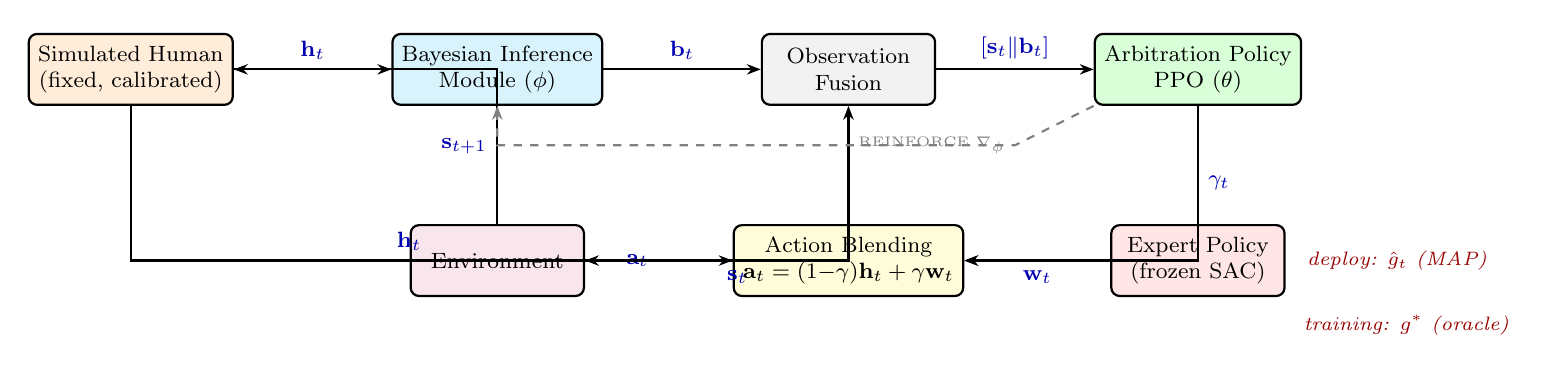
\begin{tikzpicture}[
    node distance=1.0cm and 1.4cm,
    box/.style={draw, rounded corners=3pt, minimum height=0.9cm, minimum width=2.2cm,
                font=\footnotesize, align=center, thick},
    data/.style={font=\footnotesize\itshape, text=blue!70!black},
    arrow/.style={-{Stealth[length=5pt]}, thick},
    dasharrow/.style={-{Stealth[length=5pt]}, thick, dashed, gray},
]

% Human
\node[box, fill=orange!15] (human) {Simulated Human\\(fixed, calibrated)};

% Bayesian module
\node[box, fill=cyan!15, right=2.0cm of human] (bayes) {Bayesian Inference\\Module ($\phi$)};

% Concatenation
\node[box, fill=gray!10, right=2.0cm of bayes] (concat) {Observation\\Fusion};

% PPO policy
\node[box, fill=green!15, right=2.0cm of concat] (ppo) {Arbitration Policy\\PPO ($\theta$)};

% Expert
\node[box, fill=red!10, below=1.5cm of ppo] (expert) {Expert Policy\\(frozen SAC)};

% Blending
\node[box, fill=yellow!15, below=1.5cm of concat] (blend) {Action Blending\\$\avec = (1{-}\gamma)\hvec + \gamma\wvec$};

% Environment
\node[box, fill=purple!10, below=1.5cm of bayes] (env) {Environment};

% Data labels on arrows
\draw[arrow] (human) -- node[data, above] {$\hvec$} (bayes);
\draw[arrow] (human) |- node[data, above left, pos=0.75] {$\hvec$} (blend);

\draw[arrow] (bayes) -- node[data, above] {$\bvec$} (concat);

\draw[arrow] (concat) -- node[data, above] {$[\svec \| \bvec]$} (ppo);

\draw[arrow] (ppo) -- node[data, right] {$\gamma_t$} (ppo |- blend) -- (blend);

\draw[arrow] (expert) -- node[data, below] {$\wvec$} (blend);

\draw[arrow] (blend) -- node[data, left] {$\avec$} (env);

\draw[arrow] (env) -- node[data, left] {$\mathbf{s}_{t+1}$} (env |- human) -- (human);
\draw[arrow] (env) -| node[data, below right, pos=0.25] {$\svec$} (concat);

% Gradient flow
\draw[dasharrow] (ppo.south west) -- +(-1.0, -0.5) node[font=\tiny, left, text=gray] {REINFORCE $\nabla_\phi$} -| (bayes.south);

% True goal oracle (training only)
\node[data, text=red!60!black, below right=0.15cm of expert] {\scriptsize training: $g^*$ (oracle)};
\node[data, text=red!60!black, right=0.15cm of expert.east, anchor=west] {\scriptsize deploy: $\hat{g}_t$ (MAP)};

\end{tikzpicture}
}%
\caption{BRACE data flow at each timestep.
Solid arrows: forward data flow.
Dashed arrow: gradient flow from RL objective back to belief module (Stage~2 only).
The expert receives the true goal during training (oracle) and the MAP goal at deployment.
The belief vector $\bvec$ is concatenated with the state $\svec$ to form the arbitration policy's observation.}
\label{fig:brace-dataflow}
\end{figure}


%% =================================================================
\section{Summary of Changes for Revised Manuscript}
\label{sec:changes}
%% =================================================================

Based on the above clarifications, we propose the following specific changes to the manuscript:

\begin{enumerate}
    \item \textbf{Section 3 (Methodology):} Add a formal ``Problem Setup and Notation'' subsection (before Section~3.1) that defines all variables ($\svec$, $\bvec$, $\cvec$, $\hvec$, $\wvec$, $\gamma_t$, $\avec$) with their dimensions and domains.

    \item \textbf{Section 3 (Figures 1--2):} Replace with the unified architecture diagram (Figure~\ref{fig:brace-dataflow}) that shows all variable flows, distinguishes training and deployment paths, and labels frozen vs.\ trainable components.

    \item \textbf{Section 3.1 (Training Procedure):} Expand Algorithm~1 into the detailed form of Algorithm~\ref{alg:brace-step}, making explicit that (a)~the belief conditions on raw human input $\hvec$ (not blended $\avec$), (b)~the fused observation includes the full belief vector, and (c)~the expert uses oracle goal access during training.

    \item \textbf{Section 3.1 (new subsection):} Add ``Training Data Collection and Distribution'' (content of \S\ref{sec:training-data}) explaining the two-stage process, the distributional shift between stages, and the fixed-model assumption for the simulated human.

    \item \textbf{Section 3.3 (Bayesian Inference):} Clarify that the module's three parameters ($\beta$, $w_\theta$, $w_d$) are \emph{learnable} (constrained positive via softplus) and are adapted during joint training.

    \item \textbf{Section 3.4 (Assistance Arbitration):} State explicitly that the observation is $\mathbf{o}_t = [\svec \| \bvec]$ (Eq.~\ref{eq:obs-full}) and that the policy sees the full $N$-dimensional belief vector, not a scalar summary.

    \item \textbf{Appendix C:} Expand with the concrete REINFORCE gradient (Eq.~\ref{eq:reinforce}), the mixed objective (Eq.~\ref{eq:mixed-obj}), the $\alpha$-annealing schedule, and all stabilization techniques.

    \item \textbf{New Appendix:} Add the deployment data-flow description (\S\ref{sec:deployment}), making explicit the training-to-deployment differences (MAP goal instead of oracle, real human instead of simulated).
\end{enumerate}

\end{document}
